\section{Evaluation}
\label{sec:eval}

\begin{table}[t!]
  \centering
  \caption{Server Specifications}
  \label{tab:server-specs}
  \begin{tabular}{|c|c|}
    \hline
    \textbf{Component} & \textbf{Specification} \\
    \hline
    Memory & 8x DDR4 32-GB \\
    CPU & 2x Intel Xeon E5-2630 2.4 GHz \\
    Cores per CPU & 16 \\
    L1 Cache & 512 KB \\
    L2 Cache & 2 MB \\
    L3 (LLC) Cache & 20 MB \\
    Storage & 2x 1.8 TB KVS NVMe \\
    \hline
  \end{tabular}
\end{table}

\subsection{Server Characteristics}
In \ref{tab:server-specs} we see the characteristics of our server.
The server used in our experiments is a high-performance machine with
hardware specifications found in real-world clusters.
It is equipped with 8x DDR4 32-GB 2.4 GHz 64-bit DIMMs, providing a
total of 256 GB of memory. The DDR4 memory technology is known for its
high bandwidth and low power consumption, making it ideal for
data-intensive applications like big data analytics. The server also
features Intel Xeon E5-2630 2.4 GHz 16-core 64-bit CPUs with 26 cores. 
Each core has 512 KB L1, 2 MB L2, and 20 MB L3 (LLC) cache.
The Xeon E5-2630 CPU is a high-performance processor designed for data
centers, offering a high core count, high clock speed, and advanced
features like hyper-threading and Turbo Boost. The large L3 cache
helps reduce memory latency, enabling faster data access for CPU-bound
workloads. In addition to the powerful CPUs and memory, the server
also has 2x KVS NVMe storage devices. NVMe is a high-performance
storage technology that uses PCIe to connect directly to the CPU,
providing low latency and high throughput. The KVS (Key-Value Store)
storage devices are designed for fast, random access to data, making
them ideal for storing and retrieving large amounts of data in big
data applications. Overall, the server's hardware specifications make
it a powerful platform for conducting experiments on managed big data
analytics and evaluating the performance of TeraHeap.

\subsection{Native Spark Configuration}
We use Spark v3.3.0 (\cite{Building}, \cite{Tuning}, \cite{Conf}, \cite{Monitoring}) with Kryo Serializer \cite{Kryo}, a state-of-the-art highly
optimized S/D Library for Java that Spark recommends. We run Spark
with Native OpenJDK8 \cite{JDK8} as a baseline. We use the Parallel Scavenge
garbage collector which is the one TeraHeap is implemented for.
Parallel Scavenge is also the go-to collector for applications that
need high throughput like Spark. We use one executor with 8
threads for each instance of Spark we deploy on our server \cite{TeraHeap}. Spark storage level
is configured to MEMORY-AND-DISK to place executor memory (heap) in DRAM and cache RDDs \cite{RDD}
in the on-heap cache, up to 50\% of the total heap size. Any remaining
RDDs are serialized in the off-heap cache over an NVMe SSD. This
device is also used by Spark for shuffling. 

\subsection{Native Giraph Configuration}
We run Giraph with Native OpenJDK8 \cite{JDK8} as a baseline. We use the Parallel Scavenge
garbage collector. We use one executor with 8 threads for each instance of Giraph we deploy on our server \cite{TeraHeap}. Native Giraph offloads messages and edges to the storage device.

\subsection{TeraHeap background and Spark-Giraph configurations for TeraHeap}
\subsubsection{What is TeraHeap?}
TeraHeap is a high-capacity managed heap that is memory-mapped over a
fast storage device (preferrably block-addresable NVMe or
byte-addresable NVM). The high speeds these kind of devices operate
in, erase any overhead caused by the use of MMIO. MMIO keeps the objects that reside in the storage
device deserialized, thus eliminating the need for Serialization/Deserialization  TeraHeap is designed
as an extension of the main Java Heap and is region-based. It holds specific long-lived
objects that have the same lifetime span in specific regions. This enables TeraHeap to
operate as a GC-free heap that can delete entire regions of objects at
once without the need to scan the heap over and over again for dead
objects. This would be a performance kill as it would require scans
over the storage device.

\subsubsection{Spark Configuration}
The configuration for TeraHeap is pretty much the same as for Native
Spark, with some necessary differences. TeraHeap
is mapped to a different storage device (NVMe) than that Spark is
using for shuffling. We do this in order for TeraHeap to utilize its
device to its fullest. MMIO allows TeraHeap Spark to run in
MEMORY-ONLY storage level as Spark remains unaware of using any device and
the OS takes control of the I/O.

\subsubsection{Giraph Configuration}
For Giraph we map TeraHeap to a different NVMe storage device that the one we
use for Zookeeper. TeraHeap works in the same way as in Spark
thus Giraph is unaware of the presence of a second heap.

\subsection{Experiments with single instance}

\begin{figure}[thbp]
\centering
    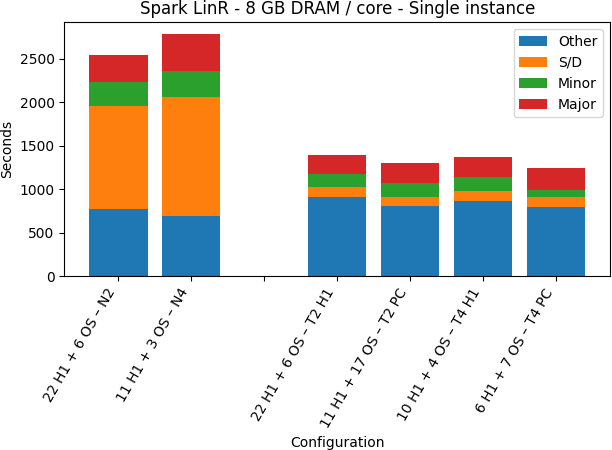
\includegraphics[width=\linewidth]{./fig/linr64_single.png}
    \caption{Execution time breakdown for single instainces of Spark
    Linear Regression. X axis shows each configuration.
        For example, 22 H1 + 6 OS - N2 is a run with two co-located instances of Native Spark (T4 for TeraHeap) with 22 GB memory for H1 and 6 for the OS to be used as Page Cache. Y axis shows execution time in seconds.}
    \label{fig:linr64_single}
    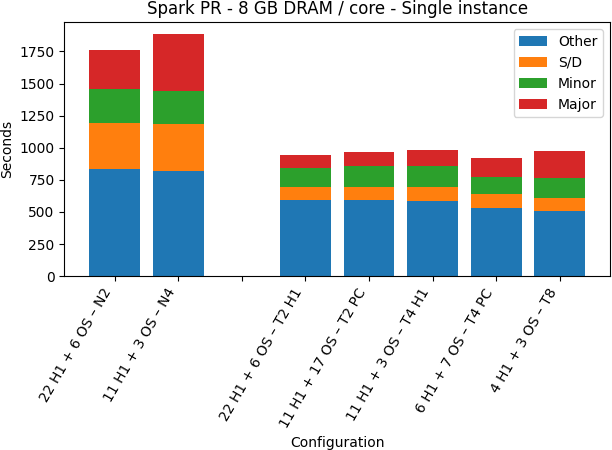
\includegraphics[width=\linewidth]{./fig/pr64_single.png}
    \caption{Execution time breakdown for single instances of Spark
    Page Rank. X axis shows each configuration.
        For example, 22 H1 + 6 OS - N2 is a run with two co-located instances of Native Spark (T4 for TeraHeap) with 22 GB memory for H1 and 6 for the OS to be used as Page Cache. Y axis shows execution time in seconds.}
    \label{fig:pr64_single}
\end{figure}

\begin{figure}[thbp]
        \centering
    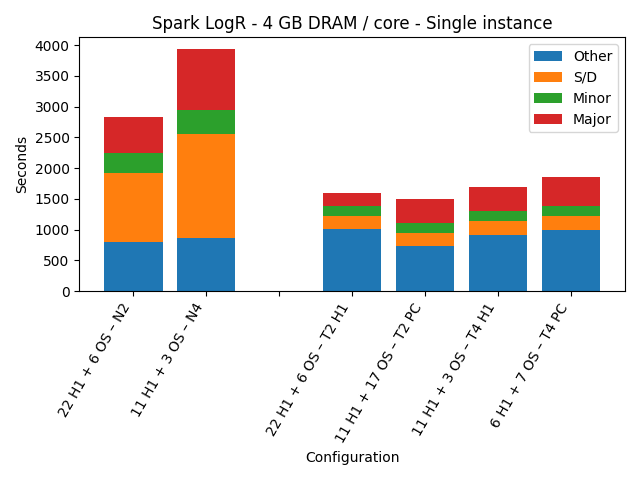
\includegraphics[width=\linewidth]{./fig/logr64_single.png}
    \caption{Execution time breakdown for single instances of Spark
    Logistic Regression. X axis shows each configuration.
        For example, 22 H1 + 6 OS - N2 is a run with two co-located instances of Native Spark (T4 for TeraHeap) with 22 GB memory for H1 and 6 for the OS to be used as Page Cache. Y axis shows execution time in seconds.}
    \label{fig:logr64_single}

    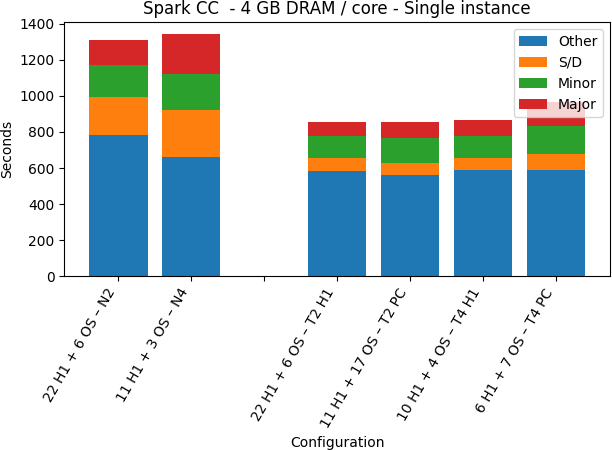
\includegraphics[width=\linewidth]{./fig/cc64_single.png}
    \caption{Execution time breakdown for single instances of Spark
    Connected Component. X axis shows each configuration.
        For example, 22 H1 + 6 OS - N2 is a run with two co-located instances of Native Spark (T4 for TeraHeap) with 22 GB memory for H1 and 6 for the OS to be used as Page Cache. Y axis shows execution time in seconds.}
    \label{fig:cc64_single}
\end{figure}

\begin{figure}[thbp]
	\iffalse
	\centering
    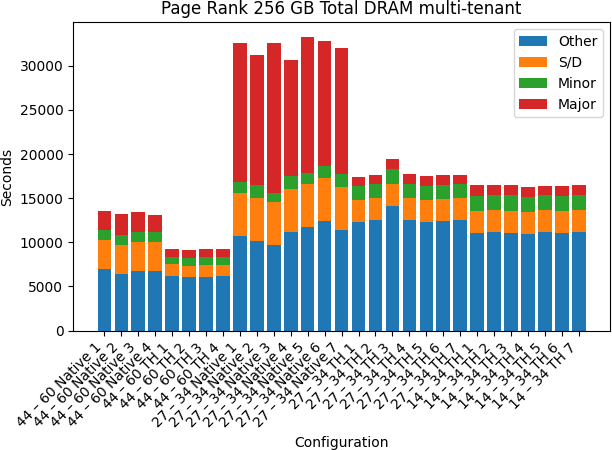
\includegraphics[width=\linewidth]{./fig/pr256.png}
    \caption{Execution time breakdown for multiple instances of Spark
    Page Rank in the 16 GB memory-per-core scenario. X axis shows each configuration.
	For example, 48 H1 + 12 OS - N4 is a run with two co-located instances of Native Spark (T4 for TeraHeap) with 48 GB memory for H1 and 12 for the OS to be used as Page Cache. Y axis shows execution time in seconds.}
    \label{fig:}
	\fi
    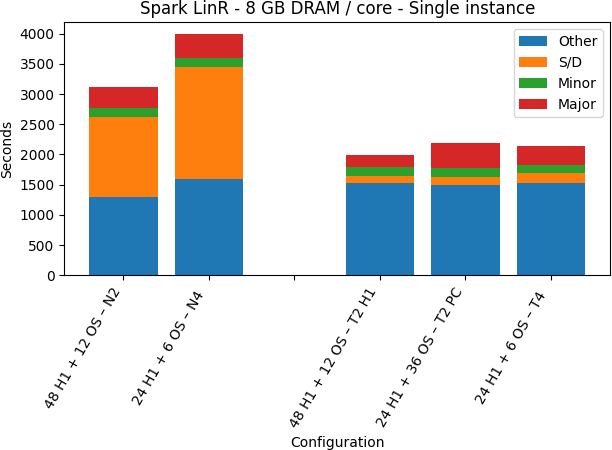
\includegraphics[width=\linewidth]{./fig/linr128_single.png}
    \caption{Execution time breakdown for single instances of Spark
    Linear Regression. X axis shows each configuration.
        For example, 48 H1 + 12 OS - N4 is a run with two co-located instances of Native Spark (T4 for TeraHeap) with 48 GB memory for H1 and 12 for the OS to be used as Page Cache. Y axis shows execution time in seconds.}
    \label{fig:linr128_single}
\end{figure}

\begin{figure}[thbp]
        \centering
    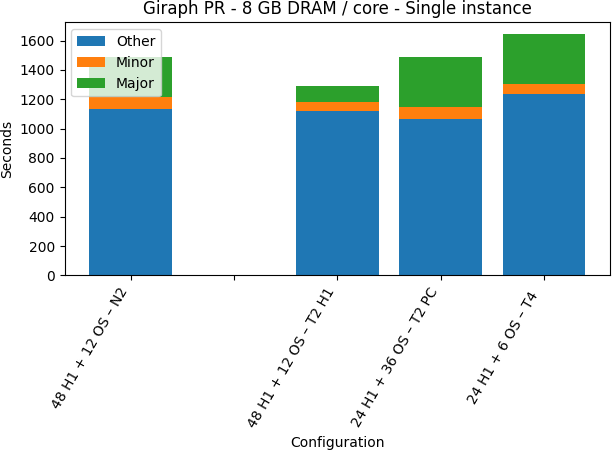
\includegraphics[width=\linewidth]{./fig/g_pr128_single.png}
    \caption{Execution time breakdown for single instances of Giraph
    Page Rank. X axis shows each configuration.
        For example, 48 H1 + 12 OS - N4 is a run with two co-located instances of Native Spark (T4 for TeraHeap) with 48 GB memory for H1 and 12 for the OS to be used as Page Cache. Y axis shows execution time in seconds.}
    \label{fig:g_pr128_single}
    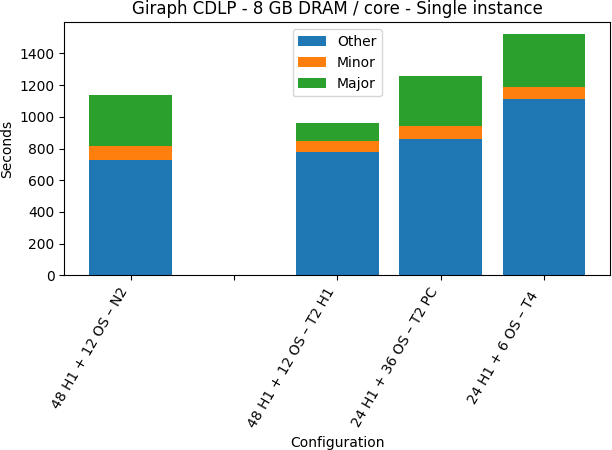
\includegraphics[width=\linewidth]{./fig/g_cdlp128_single.png}
    \caption{Execution time breakdown for single instances of Giraph
    Community Detection Label Propagation. X axis shows each configuration.
        For example, 48 H1 + 12 OS - N4 is a run with two co-located instances of Native Spark (T4 for TeraHeap) with 48 GB memory for H1 and 12 for the OS to be used as Page Cache. Y axis shows execution time in seconds.}
    \label{fig:g_cdlp128_single}
\end{figure}

Figure \ref{fig:pr64_single} shows single instance performance with Page Rank for Native and TH Spark. These experiments correspond to the co-located runs of figure \ref{fig:pr64}. The first two bars show performance of Native Spark for 28 and 14 GB DRAM. When H1 decreases Native suffers from longer and more frequent GC cycles thus we see an increment to Major GC. S/D and other time remain the same as Read/Write traffic remains the same. The rest four bars show performance for TH Spark for 28 (80\% and 40\% for H1) and 14 (80\% and 40\% for H1) GB DRAM. As we said in our methodology, for TeraHeap we investigate setups with DRAM budgets where both H1 and PC dominate. For Native we saw no differences with variable Page Cache sizes for any of the experiments thus we do not show them here. As H1 decreases for TeraHeap we see an increase to Major GC in the last 2 bars. Other time and S/D remain the same.

Figure \ref{fig:linr64_single} shows single instance performance with Linear Regression for Native and TH Spark. These experiments correspond to the co-located runs of figure \ref{fig:linr64}. The first two bars show performance of Native Spark for 28 and 14 GB DRAM. When H1 decreases Native suffers from longer and more frequent GC cycles thus we see an increment to Major GC. S/D has a slight increase because of increased Read traffic caused by memory pressure. Write traffic remains the same because objects in Spark are immutable. The rest four bars show performance for TH Spark for 28 (80\% and 40\% for H1) and 14 (80\% and 40\% for H1) GB DRAM. For Native we saw no differences with variable Page Cache sizes for any of the experiments thus we do not show them here. As H1 decreases for TeraHeap we see an increase to Major GC in the last 2 bars. Other time shows slight differences because of cache size. That can be seen from the second and third bar which have the same amount for H1 and a big difference in cache. S/D remains the same.

Figure \ref{fig:logr64_single} shows single instance performance with Logistic Regression for Native and TH Spark. These experiments correspond to the co-located runs of figure \ref{fig:logr64}. The first two bars show performance of Native Spark for 28 and 14 GB DRAM. When H1 decreases Native suffers from longer and more frequent GC cycles thus we see a significant increment to Major GC. S/D has a huge increase of almos 30\% because of increased read traffic caused by memory pressure. Write traffic remains the same because objects in Spark are immutable. The rest four bars show performance for TH Spark for 28 (80\% and 40\% for H1) and 14 (80\% and 40\% for H1) GB DRAM. For Native we saw no differences with variable Page Cache sizes for any of the experiments thus we do not show them here. As H1 decreases for TeraHeap we see some notable differences to GC. Other time shows differences because of cache size. That can be seen from the second and third bar which have the same amount for H1 and a big difference in cache. That can be seen from the second and third bar which have the same amount for H1 and a big difference in cache. S/D remains the same.

Figure \ref{fig:cc64_single} shows single instance performance with Connected Component for Native and TH Spark. These experiments correspond to the co-located runs of figure \ref{fig:cc64}. The first two bars show performance of Native Spark for 28 and 14 GB DRAM. When H1 decreases Native suffers from longer and more frequent GC cycles thus we see an increment to Major GC. S/D has a huge increase of almost 50\% because of increased read traffic caused by memory pressure. Write traffic remains the same because objects in Spark are immutable. The rest four bars show performance for TH Spark for 28 (80\% and 40\% for H1) and 14 (80\% and 40\% for H1) GB DRAM. For Native we saw no differences with variable Page Cache sizes for any of the experiments thus we do not show them here. As H1 decreases for TeraHeap we see an increase to Minor GC in the last bar. Other time and S/D remain the same.

Figure \ref{fig:linr128_single} shows single instance performance with Linear Regression for Native and TH Spark. These experiments correspond to the co-located runs of figure \ref{fig:linr128}. The first two bars show performance of Native Spark for 60 and 30 GB DRAM. When H1 decreases Native suffers from longer and more frequent GC cycles thus we see an increment to Major GC. S/D has a slight increase because of increased Read traffic caused by memory pressure. Write traffic remains the same because objects in Spark are immutable. The rest four bars show performance for TH Spark for 60 (80\% and 40\% for H1) and 30 (80\% and 40\% for H1) GB DRAM. For Native we saw no differences with variable Page Cache sizes for any of the experiments thus we do not show them here. As H1 decreases for TeraHeap we see an increase to Major GC. Other time shows slight differences because of cache size. S/D remains the same.

Figure \ref{fig:g_pr128_single} shows single instance performance with Page Rank for Native and TH Giraph. These experiments correspond to the co-located runs of figure \ref{fig:g_pr128}. The first bar shows performance of Native Giraph for 60 GB DRAM. The rest three bars show performance for TH Giraph for 60 (80\% and 40\% for H1) and 30 (80\% for H1) GB DRAM. For Native we saw no differences with variable Page Cache sizes for any of the experiments thus we do not show them here. As H1 decreases for TeraHeap we see an increase to Major GC  and Other time. Other time changes by both H1 and Page Cache differences. We see that H1 affects writes in a significant way because objects are mutable in Giraph and decreasing H1 creates more traffic to TeraHeap. Page Cache mostly affects read traffic. These can be seen from the progression of the bars in other time.

Figure \ref{fig:g_cdlp128_single} shows single instance performance with Page Rank for Native and TH Giraph. These experiments correspond to the co-located runs of figure \ref{fig:g_pr128}. The first bar shows performance of Native Giraph for 60 GB DRAM. The rest three bars show performance for TH Giraph for 60 (80\% and 40\% for H1) and 30 (80\% for H1) GB DRAM. For Native we saw no differences with variable Page Cache sizes for any of the experiments thus we do not show them here. As H1 decreases for TeraHeap we see an increase to Major GC  and Other time. Other time changes by both H1 and Page Cache differences. We see that H1 affects writes in a significant way because objects are mutable in Giraph and decreasing H1 creates more traffic to TeraHeap. Page Cache mostly affects read traffic. These can be seen from the progression of the bars in other time.


\subsection{Experiments with colocated instances}

\begin{figure}[thbp]
\centering
    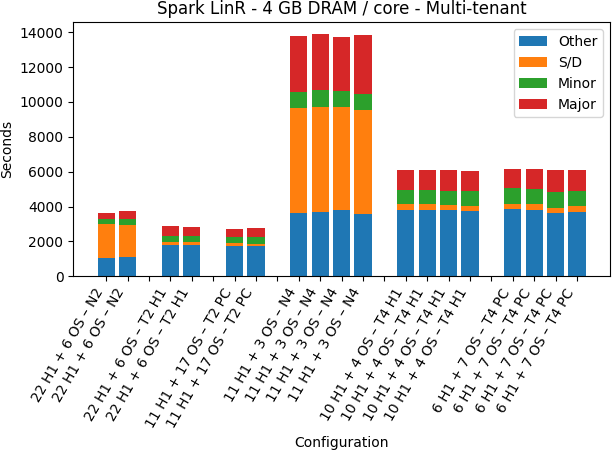
\includegraphics[width=\linewidth]{./fig/linr64.png}
    \caption{Execution time breakdown for co-located instances of Spark
    Linear Regression in the 4 GB memory-per-core scenario. X axis shows each configuration.
        For example, 22 H1 + 6 OS - N2 is a run with two co-located instances of Native Spark (T4 for TeraHeap) with 22 GB memory for H1 and 6 for the OS to be used as Page Cache. Y axis shows execution time in seconds.}
    \label{fig:linr64}
    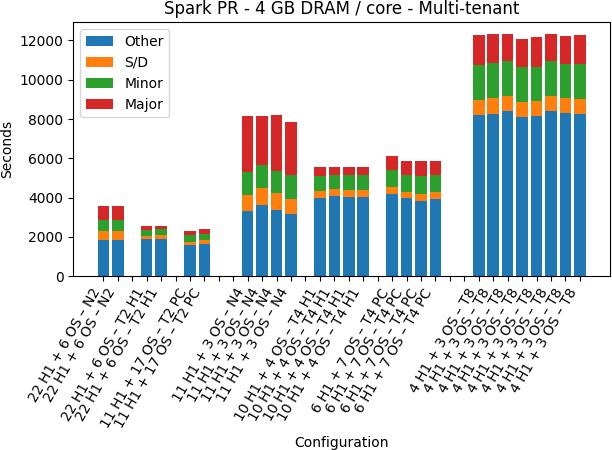
\includegraphics[width=\linewidth]{./fig/pr64.png}
    \caption{Execution time breakdown for co-located instances of Spark
    Page Rank in the 4 GB memory-per-core scenario. X axis shows each configuration.
        For example, 22 H1 + 6 OS - N2 is a run with two co-located instances of Native Spark (T4 for TeraHeap) with 22 GB memory for H1 and 6 for the OS to be used as Page Cache. Y axis shows execution time in seconds.}
    \label{fig:pr64}
\end{figure}

\begin{figure}[thbp]
        \centering
    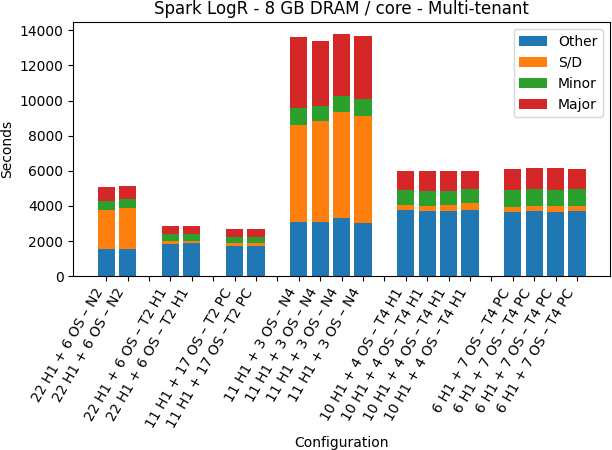
\includegraphics[width=\linewidth]{./fig/logr64.png}
    \caption{Execution time breakdown for co-located instances of Spark
    Logistic Regression in the 4 GB memory-per-core scenario. X axis shows each configuration.
        For example, 22 H1 + 6 OS - N2 is a run with two co-located instances of Native Spark (T4 for TeraHeap) with 22 GB memory for H1 and 6 for the OS to be used as Page Cache. Y axis shows execution time in seconds.}
    \label{fig:logr64}

    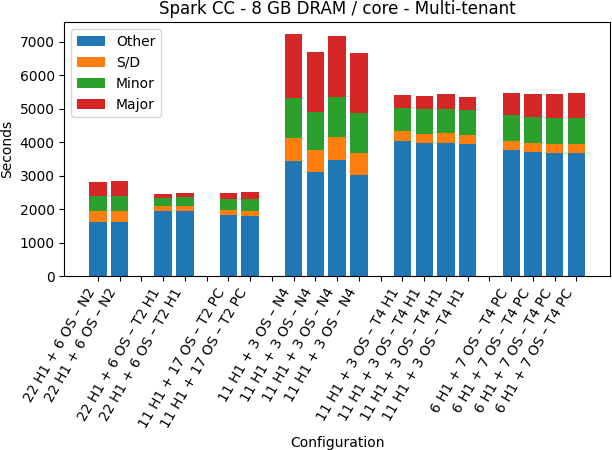
\includegraphics[width=\linewidth]{./fig/cc64.png}
    \caption{Execution time breakdown for co-located instances of Spark
    Connected Component in the 4 GB memory-per-core scenario. X axis shows each configuration.
        For example, 22 H1 + 6 OS - N2 is a run with two co-located instances of Native Spark (T4 for TeraHeap) with 22 GB memory for H1 and 6 for the OS to be used as Page Cache. Y axis shows execution time in seconds.}
    \label{fig:cc64}
\end{figure}

\begin{figure}[thbp]
	\iffalse
        \centering
    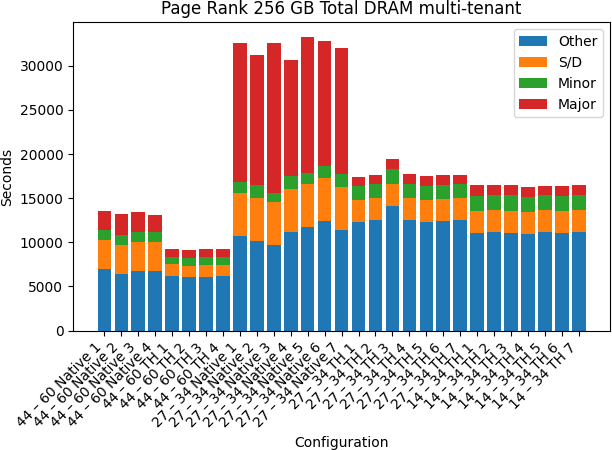
\includegraphics[width=\linewidth]{./fig/pr256.png}
    \caption{Execution time breakdown for co-located instances of Spark
    Page Rank in the 16 GB memory-per-core scenario. X axis shows each configuration.
        For example, 48 H1 + 12 OS - N4 is a run with two co-located instances of Native Spark (T4 for TeraHeap) with 48 GB memory for H1 and 12 for the OS to be used as Page Cache. Y axis shows execution time in seconds.}
    \label{fig:pr256}
	\fi
    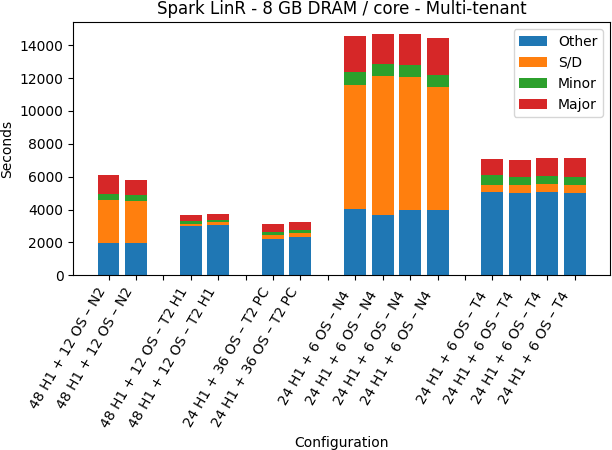
\includegraphics[width=\linewidth]{./fig/linr128.png}
    \caption{Execution time breakdown for co-located instances of Spark
    Linear Regression in the 8 GB memory-per-core scenario. X axis shows each configuration.
        For example, 48 H1 + 12 OS - N4 is a run with two co-located instances of Native Spark (T4 for TeraHeap) with 48 GB memory for H1 and 12 for the OS to be used as Page Cache. Y axis shows execution time in seconds.}
    \label{fig:linr128}
\end{figure}

\begin{figure}[thbp]
        \centering
    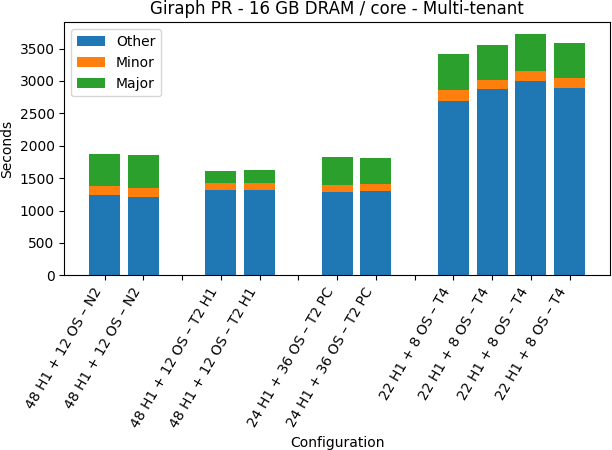
\includegraphics[width=\linewidth]{./fig/g_pr128.png}
    \caption{Execution time breakdown for co-located instances of Giraph
    Page Rank in the 8 GB memory-per-core scenario. X axis shows each configuration.
        For example, 48 H1 + 12 OS - N4 is a run with two co-located instances of Native Spark (T4 for TeraHeap) with 48 GB memory for H1 and 12 for the OS to be used as Page Cache. Y axis shows execution time in seconds.}
    \label{fig:g_pr128}
    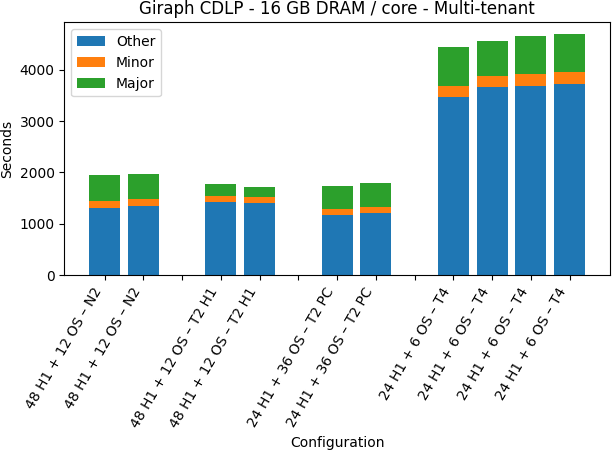
\includegraphics[width=\linewidth]{./fig/g_cdlp128.png}
    \caption{Execution time breakdown for co-located instances of Giraph
    Community Detection Label Propagation in the 8 GB memory-per-core scenario. X axis shows each configuration.
        For example, 48 H1 + 12 OS - N4 is a run with two co-located instances of Native Spark (T4 for TeraHeap) with 48 GB memory for H1 and 12 for the OS to be used as Page Cache. Y axis shows execution time in seconds.}
    \label{fig:g_cdlp128}
\end{figure}


Here we look at the co-located experiments of Spark and Giraph in all memory-per-core categories.
Any runs that are not shown should be considered experiments that run Out of memory (OOM) for H1.
LinR and LogR experiments with 10 GB H1 out of 14 GB cgroup DRAM budget which is less than 80\% were conducted this way
because less than 4 GB available memory for the OS caused the cgroup to stop execution resulting to OOM error.

We explain each figure from 4 aspects:
\begin{itemize}
\item{The differences in the time breakdown while number of instances increase for each configuration.}
\item{A comparison between the different configurations while instances increase.}
\item{A comparison with the single instance experiment}
\item{A comparison between H1 and Page Cache dominating configurations}
\end{itemize}

\subsubsection{4 GB DRAM / core}

Figure \ref{fig:linr64} shows the performance of multiple
Native-TeraHeap Spark instances running LinearRegression with 64 GB
dataset per instance in our 64 GB DRAM machine. Each instance of Spark
uses one executor with 8 cores per executor. Available DRAM is 56 GB
and 8 GB are left to the Operating system, resulting in 64 GB total
DRAM. All configurations utilize 56 of 64 GB total DRAM. 
Starting from the left of the graph, the first 6 bars show the
performance of 3 runs. The first run is with 2 colocated Native Spark instances.
Another run with 2 colocated TH Spark instances with H1 dominating Page Cache
and a third run with 2 colocated TH Spark instances where Page Cache dominates H1. 
Each instance of the first 2 runs uses 22 GB DRAM for H1 (Java Heap) and 6 GB for rest of the services.
The third run uses 11 GB DRAM for H1 and 17 GB for Page Cache for each instance. 
The rest 12 bars show the performance of another 3 runs. The first run is with 4 colocated Native Spark instances.
Another run with 4 colocated TH Spark instances with H1 dominating Page Cache
and a third run with 4 colocated TH Spark instances where Page Cache dominates H1. 
Each instance of the first run uses 11 GB DRAM for H1 (Java Heap) and 3 GB for rest of the services. 
The second run uses 10 GB DRAM for H1 and 4 GB for Page Cache for each instance. 
The third run uses 6 GB DRAM for H1 and 8 GB for Page Cache for each instance. 
Considering the first aspect we see that GC and S/D increase dramatically for Native Spark along with significant increase to Other time. GC differences are witnessed because the heap capacity decreases and that causes memory pressure. TeraHeap Spark shows a slight increase to Major GC while the number of instances increases. This is because of the decreased heap capacity. For Native Spark 2 co-located instances have 71\% speedup in execution time compared to 4 co-located instances and provide 46\% more average throughput. For TH H1 2 co-located instances have 50\% speedup in execution time compared to 4 co-located instances and provide 8\% more average throughput. For TH PC performance is the same with TH H1. 
S/D is completely absorbed by MMIO. From the third aspect, as instances increase in the server the benefit gap between Native and TeraHeap Spark becomes bigger. As Native Spark starves from more GC and S/D, TeraHeap maintains its benefits. That is shown by the speedups where TeraHeap has 25\% and 57\% speedup and 48\% and 66\% more average throughput for 2 and 4 instances when compared to the corresponding Native runs.

Figure \ref{fig:pr64} shows the performance of multiple
Native-TeraHeap Spark instances running PageRank with 8 GB
dataset per instance in our 64 GB DRAM machine. Each instance of Spark
uses one executor with 8 cores per executor. Available DRAM is 56 GB
and 8 GB are left to the Operating system, resulting in 64 GB total
DRAM. All configurations utilize 56 of 64 GB total DRAM.
Starting from the left of the graph, the first 6 bars show the
performance of 3 runs. The first run is with 2 colocated Native Spark instances.
Another run with 2 colocated TH Spark instances with H1 dominating Page Cache
and a third run with 2 colocated TH Spark instances where Page Cache dominates H1.
Each instance of the first 2 runs uses 22 GB DRAM for H1 (Java Heap) and 6 GB for rest of the services.
The third run uses 11 GB DRAM for H1 and 17 GB for Page Cache for each instance. 
The next 12 bars show the performance of another 3 runs. The first run is with 4 colocated Native Spark instances.
Another run with 4 colocated TH Spark instances with H1 dominating Page Cache
and a third run with 4 colocated TH Spark instances where Page Cache dominates H1.
Each instance of the first run uses 11 GB DRAM for H1 (Java Heap) and 3 GB for rest of the services.
The second run uses 10 GB DRAM for H1 and 4 GB for Page Cache for each instance.
The third run uses 6 GB DRAM for H1 and 8 GB for Page Cache for each instance.
The last 8 bars refer to 8 colocated instances of TeraHeap Spark only. 
We were unable to decrease H1 enough to run 8 colocates instance of Native Spark
because JVM runs out of memory. Each instance of the run uses 4 GB DRAM for H1 (Java Heap) and 3 GB for Page Cache.
Considering the first aspect we see that Minor and Major GC increase dramatically for Native Spark along with significant increase to Other time. Minor and Major GC differences are witnessed because the heap capacity decreases and that causes memory pressure. TeraHeap Spark shows a slight increase to Major GC while the number of instances increases. This is because of the decreasing heap capacity. Other time increases because more objects are moved to TeraHeap but this is a good trade-off because all the GC is absorbed. S/D is completely absorbed by MMIO. 
For Native Spark 2 co-located instances have 55\% speedup in execution time compared to 4 co-located instances and provide 20\% more average throughput. For TH H1 2 co-located instances have 40\% speedup in execution time compared to 4 co-located instances and provide 14\% more average throughput. For TH PC performance is the same with TH H1. For TH 8 co-located instances have 50 and 83\% speedup against 4 and 2 instances accordingly.
From the second aspect, as instances increase in the server the benefit gap between Native and TeraHeap Spark becomes bigger. As Native Spark starves from more GC and S/D, TeraHeap maintains its benefits. TeraHeap has 50 and 25\% speedup for 2 and 4 instances when compared to the corresponding Native runs. If we compare TeraHeap 8 instances to the 4 instances of Native TeraHeap has 33\% worse performance but 33\% more average throughput.

Figure \ref{fig:logr64} shows the performance of multiple
Native-TeraHeap Spark instances running Logistic Regression with 64 GB
dataset per instance in our 64 GB DRAM machine. Each instance of Spark
uses one executor with 8 cores per executor. Available DRAM is 56 GB
and 8 GB are left to the Operating system, resulting in 64 GB total
DRAM. All configurations utilize 56 of 64 GB total DRAM.
Starting from the left of the graph, the first 6 bars show the
performance of 3 runs. The first run is with 2 colocated Native Spark instances.
Another run with 2 colocated TH Spark instances with H1 dominating Page Cache
and a third run with 2 colocated TH Spark instances where Page Cache dominates H1.
Each instance of the first 2 runs uses 22 GB DRAM for H1 (Java Heap) and 6 GB for rest of the services.
The third run uses 11 GB DRAM for H1 and 17 GB for Page Cache for each instance. 
The next 12 bars show the performance of another 3 runs. The first run is with 4 colocated Native Spark instances.
Another run with 4 colocated TH Spark instances with H1 dominating Page Cache
and a third run with 4 colocated TH Spark instances where Page Cache dominates H1.
Each instance of the first run uses 11 GB DRAM for H1 (Java Heap) and 3 GB for rest of the services.
The second run uses 10 GB DRAM for H1 and 4 GB for Page Cache for each instance.
The third run uses 6 GB DRAM for H1 and 8 GB for Page Cache for each instance.
Considering the first aspect we see that GC and S/D increase dramatically for Native Spark along with significant increase to Other time. GC differences are witnessed because the heap capacity decreases and that causes memory pressure. TeraHeap Spark shows a slight increase to Major GC while the number of instances increases. This is because of the decreased heap capacity. Other time increases because more objects are moved to TeraHeap and read/write traffic increases but this is a good trade-off because all the GC is absorbed. S/D is completely absorbed by MMIO. For Native Spark 2 co-located instances have 62\% speedup in execution time compared to 4 co-located instances and provide 27\% more average throughput. For TH H1 2 co-located instances have 50\% speedup in execution time compared to 4 co-located instances and provides the same throughput. For TH PC performance is the same with TH H1. From the second aspect, as instances increase in the server the benefit gap between Native and TeraHeap Spark becomes bigger. As Native Spark starves from more GC and S/D, TeraHeap maintains its benefits. TeraHeap has 57 and 40\% speedup and 48\% and 66\% increased average throughputfor 2 and 4 instances when compared to the corresponding Native runs.

Figure \ref{fig:cc64} shows the performance of multiple
Native-TeraHeap Spark instances running Connected Component with 8 GB
dataset per instance in our 64 GB DRAM machine. Each instance of Spark
uses one executor with 8 cores per executor. Available DRAM is 56 GB
and 8 GB are left to the Operating system, resulting in 64 GB total
DRAM. All configurations utilize 56 of 64 GB total DRAM.
Starting from the left of the graph, the first 6 bars show the
performance of 3 runs. The first run is with 2 colocated Native Spark instances.
Another run with 2 colocated TH Spark instances with H1 dominating Page Cache
and a third run with 2 colocated TH Spark instances where Page Cache dominates H1.
Each instance of the first 2 runs uses 22 GB DRAM for H1 (Java Heap) and 6 GB for rest of the services.
The third run uses 11 GB DRAM for H1 and 17 GB for Page Cache for each instance. 
The next 12 bars show the performance of another 3 runs. The first run is with 4 colocated Native Spark instances.
Another run with 4 colocated TH Spark instances with H1 dominating Page Cache
and a third run with 4 colocated TH Spark instances where Page Cache dominates H1.
Each instance of the first run uses 11 GB DRAM for H1 (Java Heap) and 3 GB for rest of the services.
The second run uses 10 GB DRAM for H1 and 4 GB for Page Cache for each instance.
The third run uses 6 GB DRAM for H1 and 8 GB for Page Cache for each instance.
Considering the first aspect we see that Minor and Major GC increase dramatically for Native Spark along with significant increase to Other time. Minor and Major GC differences are witnessed because the heap capacity decreases and that causes memory pressure. TeraHeap Spark shows a slight increase to Major GC while the number of instances increases. This is because of the decreasing heap capacity. Other time increases because more objects are moved to TeraHeap but this is a good trade-off because all the GC is absorbed. S/D is completely absorbed by MMIO. For Native Spark 2 co-located instances have 57\% speedup in execution time compared to 4 co-located instances and provide 27\% more average throughput. For TH H1 2 co-located instances have 54\% speedup in execution time compared to 4 co-located instances and provides 8\% less throughput.
From the second aspect, as instances increase in the server the benefit gap between Native and TeraHeap Spark becomes bigger. As Native Spark starves from more GC and S/D, TeraHeap maintains its benefits. TeraHeap has 21 and 15\% speedup and 10\% more throughput for 2 and 4 instances when compared to the corresponding Native runs.

\subsubsection{8 GB DRAM / core}

Figure \ref{fig:linr128} shows the performance of multiple
Native-TeraHeap Spark instances running LinearRegression with 128 GB
dataset per instance in our 128 GB DRAM machine.
Starting from the left of the graph, the first 6 bars show the
performance of 3 runs. The first run is with 2 colocated Native Spark instances.
Another run with 2 colocated TH Spark instances with H1 dominating Page Cache
and a third run with 2 colocated TH Spark instances where Page Cache dominates H1.
Each instance of the first 2 runs uses 48 GB DRAM for H1 (Java Heap) and 12 GB for rest of the services.
The third run uses 24 GB DRAM for H1 and 36 GB for Page Cache for each instance.
The rest 8 bars show the performance of another 2 runs. The first run is with 4 colocated Native Spark instances.
Another run with 4 colocated TH Spark instances with H1 dominating Page Cache
and a third run with 4 colocated TH Spark instances where Page Cache dominates H1.
Each instance of the first run uses 24 GB DRAM for H1 (Java Heap) and 6 GB for rest of the services.
The second run uses 24 GB DRAM for H1 and 6 GB for Page Cache for each instance.
Considering the first aspect we see that GC and S/D increase dramatically for TeraHeap Spark along with significant increase to Other time. GC differences are witnessed because the heap capacity decreases and that causes memory pressure. TeraHeap Spark shows a slight increase to Major GC while the number of instances increases. This is because of the decreased heap capacity. For Native Spark 2 co-located instances have 57\% speedup in execution time compared to 4 co-located instances and provide 18\% more average throughput. For TH H1 2 co-located instances have 50\% speedup in execution time compared to 4 co-located instances and provide the same average throughput. For TH PC 2 co-located instances have 50\% speedup in execution time compated to 4 co-located instances and provide the same average throughput. 
S/D is completely absorbed by MMIO. From the second aspect, as instances increase in the server the benefit gap between Native and TeraHeap Spark becomes bigger. As Native Spark starves from more GC and S/D, TeraHeap maintains its benefits. That is shown by the speedups where TeraHeap has 50\% speedup and 73\% and 77\% more average throughput for 2 and 4 instances when compared to the corresponding Native runs.

Figure \ref{fig:g_pr128} shows the performance of multiple
Native-TeraHeap Giraph instances running Page Rank with 13 GB
dataset per instance in our 128 GB DRAM machine.
Starting from the left of the graph, the first 6 bars show the
performance of 3 runs. The first run is with 2 colocated Native Giraph instances.
Another run with 2 colocated TH Giraph instances with H1 dominating Page Cache
and a third run with 2 colocated TH Instances instances where Page Cache dominates H1.
Each instance of the first 2 runs uses 48 GB DRAM for H1 (Java Heap) and 12 GB for rest of the services.
The third run uses 24 GB DRAM for H1 and 36 GB for Page Cache for each instance.
The rest 4 bars show the performance of another run. The run is with 4 colocated TeraHeap Giraph instances.
Each instance uses 24 GB DRAM for H1 (Java Heap) and 6 GB for rest of the services.
Considering the first aspect Native Giraph does not scale to 4 instances and runs out of memory. TeraHeap Giraph shows significant increase to Major GC while the number of instances increases. This is because of the decreased heap capacity. For TH H1 2 co-located instances have 57\% speedup in execution time compared to 4 co-located instances and provide the same average throughput. For TH PC 2 co-located instances have 51\% speedup in execution time compated to 4 co-located instances and provide the same average throughput.
From the second aspect, TeraHeap is able to scale to 4 instances while Native runs out of memory. TeraHeap has 11\% speedup and 13\% more average throughput for 2 instances when compared to the corresponding Native runs.

Figure \ref{fig:g_cdlp128} shows the performance of multiple
Native-TeraHeap Giraph instances running CDLP with 13 GB
dataset per instance in our 128 GB DRAM machine.
Starting from the left of the graph, the first 6 bars show the
performance of 3 runs. The first run is with 2 colocated Native Giraph instances.
Another run with 2 colocated TH Giraph instances with H1 dominating Page Cache
and a third run with 2 colocated TH Instances instances where Page Cache dominates H1.
Each instance of the first 2 runs uses 48 GB DRAM for H1 (Java Heap) and 12 GB for rest of the services.
The third run uses 24 GB DRAM for H1 and 36 GB for Page Cache for each instance.
The rest 4 bars show the performance of another run. The run is with 4 colocated TeraHeap Giraph instances.
Each instance uses 24 GB DRAM for H1 (Java Heap) and 6 GB for rest of the services.
Considering the first aspect Native Giraph does not scale to 4 instances and runs out of memory. TeraHeap Giraph shows significant increase to Major GC while the number of instances increases. This is because of the decreased heap capacity. For TH H1 2 co-located instances have 63\% speedup in execution time compared to 4 co-located instances and provide 27\% more average throughput. For TH PC 2 co-located instances have 61\% speedup in execution time compared to 4 co-located instances and 27\% more average throughput. From the second aspect, TeraHeap is able to scale to 4 instances while Native runs out of memory. TeraHeap has 9\% speedup and 7\% more average throughput for 2 instances when compared to the corresponding Native runs.

\iffalse
\subsubsection{16 GB DRAM / core}

Figure \ref{fig:pr256} shows the performance of multiple
Native-TeraHeap Spark instances running PageRank with 32 GB
dataset per instance in our 256 GB DRAM machine.
The graph, shows the
performance of 3 runs. The first run is with 4 colocated Native Spark instances.
Another run with 4 colocated TH Spark instances with H1 dominating Page Cache.
Each instance of the first 8 runs uses 48 GB DRAM for H1 (Java Heap) and 12 GB for rest of the services including Page Cache.
Each instance of the first run uses 27 GB DRAM for H1 (Java Heap) and 7 GB for rest of the services.
The second run uses 27 GB DRAM for H1 and 7 GB for Page Cache for each TH instance.
The third run uses 14 GB DRAM for H1 and 20 GB for Page Cache for each TH instance.
Considering the first aspect we see that GC and S/D increase dramatically for TeraHeap Spark along with significant increase to Other time. GC differences are witnessed because the heap capacity decreases and that causes memory pressure. TeraHeap Spark shows a slight increase to Minor GC while the number of instances increases. This is because of the decreased heap capacity. For Native Spark 2 co-located instances have 57\% speedup in execution time compared to 4 co-located instances and provide 18\% more average throughput. For TH H1 2 co-located instances have 50\% speedup in execution time compared to 4 co-located instances and provide the same average throughput. For TH PC 2 co-located instances have 50\% speedup in execution time compated to 4 co-located instances and provide the same average throughput. So choosing H1 or PC setup for TH does not make any up or downsides. Native PC setup is not shown in the figure because PC does not have any impact and decreasing H1 would obviously downgrade performance compared to Native H1.
S/D is completely absorbed by MMIO. From the third aspect, as instances increase in the server the benefit gap between Native and TeraHeap Spark becomes bigger. As Native Spark starves from more GC and S/D, TeraHeap maintains its benefits. That is shown by the speedups where TeraHeap has 50\% speedup and 73\% and 77\% more average throughput for 2 and 4 instances when compared to the corresponding Native runs.
\fi

\subsubsection{Interference with single instance}

\begin{table}[thbp]
  \centering
  \caption{Interference for each configuration with co-located instances with corresponding single instance experiment.
	FW = framework, Conf. = configuration, M/C = Memory/core, #I = Number of instances, Interf. = interference }
  \label{tab:interference}
  \begin{tabular}{|c|c|c|c|c|}
    \hline
	  \textbf{FW} & \textbf{Conf.} & \textbf{M/C (GB)} & \textbf{\#I} & \textbf{Interf. \%} \\
    \hline
	  Spark & PR Native & 4 & 2 & 51 \\
	  Spark & PR Native & 4 & 4 & 77 \\
	  Spark & PR TH H1 & 4 & 2 &  63 \\
	  Spark & PR TH PC & 4 & 2 & 59 \\
	  Spark & PR TH H1 & 4 & 4 &  82 \\
	  Spark & PR TH PC & 4 & 4 & 84 \\
	  Spark & PR TH & 4 & 8 & 92 \\
	  Spark & LINR Native & 4 & 2 & 32  \\
	  Spark & LINR Native & 4 & 4 & 80 \\
	  Spark & LINR TH H1 & 4 & 2 & 52 \\
	  Spark & LINR TH PC & 4 & 2 & 53 \\
	  Spark & LINR TH H1 & 4 & 4 & 78 \\
	  Spark & LINR TH PC & 4 & 4 & 80 \\
	  Spark & LINR Native & 8 & 2 & 49 \\
	  Spark & LINR Native & 8 & 4 & 73 \\
	  Spark & LINR TH H1 & 8 & 2 & 46 \\
	  Spark & LINR TH PC & 8 & 2 & 32 \\
	  Spark & LINR TH H1 & 8 & 4 & 71 \\
	  Spark & LINR TH PC & 8 & 4 & 73 \\
	  Spark & LOGR Native & 4 & 2 & 45 \\
	  Spark & LOGR Native & 4 & 4 & 71 \\
	  Spark & LOGR TH H1 & 4 & 2 & 44 \\
	  Spark & LOGR TH PC & 4 & 2 & 44 \\
	  Spark & LOGR TH H1 & 4 & 4 & 73 \\
	  Spark & LOGR TH PC & 4 & 4 & 75 \\
          Spark & CC Native & 4 & 2 & 56 \\
          Spark & CC Native & 4 & 4 & 75 \\
          Spark & CC TH H1 & 4 & 2 & 66 \\
          Spark & CC TH PC & 4 & 2 & 66 \\
          Spark & CC TH H1 & 4 & 4 & 84  \\
          Spark & CC TH PC & 4 & 4 & 76 \\
          Giraph & PR Native & 8 & 2 & 19 \\
          Giraph & PR TH H1 & 8 & 2 & 21 \\
          Giraph & PR TH PC & 8 & 2 & 38 \\
          Giraph & PR TH & 8 & 4 & 55 \\
          Giraph & CDLP Native & 8 & 2 & 41 \\
          Giraph & CDLP TH H1 & 8 & 2 & 45 \\
          Giraph & CDLP TH PC & 8 & 2 & 30 \\
          Giraph & CDLP TH & 8 & 4 & 67 \\
    \hline
  \end{tabular}
\end{table}

Table \ref{tab:interference} shows the percentage of interference i.e. speedup of single instance against the corresponding co-located experiment. For Native Spark for 2 to 4 co-located instances experiments there is 32 to 80\% interference. For TeraHeap Spark for 2 to 4 co-located instances experiments there is 32 to 84\% interference. Both offloading techniques have the same interference ranges which are more than 50\% in most of the experiments. For Native Giraph there is 19\% interference for PR and 41\% for CDLP with 2 co-located instances. The first is really reduced compared to the Native Spark 2 co-located instances experiments. For TH Giraph there is 21 to 67 \% interference. For 4 co-located instances experiments TH Giraph has significantly less interference than Spark. 

\subsubsection{Does H1 or PageCache offer better performance?}
We don't investigate Page Cache-dominated cgroup budgets since we have seen that it does not make a difference for Spark or Giraph. For TeraHeap Spark Page Cache provides slightly better average throughput for 2 co-located instances for 4 instances H1 dominates PC. For TeraHeap Giraph, H1 dominates PC in terms of average throughput. That is because H1 affects Write traffic in Giraph and Page Cache absorbs mostly reads.

\subsubsection{Accuracy of experiments}

We repeated all experiments with 1,2 and 4 instances except TH with PC and TH with 8 instances for PR a second time to estimate standard deviation. We left there experiments out because of lack of time. Table \ref{tab:std-dev} shows that 
all experiments have less than 5\% standard deviation. Also co-located experiments have under 7\% difference in-between the end of execution of each co-located instance. This is important because when one instance has finished the interference decreases.

\begin{table}[thbp]
  \centering
  \caption{Standard deviation for each configuration and number of co-located instances.
	FW=framework, Conf. = configuration, M/C = memory/core, #I=number of instances, St. dev.=standard deviation}
  \label{tab:std-dev}
  \begin{tabular}{|c|c|c|c|c|}
    \hline
	  \textbf{FW} & \textbf{Conf.} & \textbf{M/C (GB)} & \textbf{\#I} & \textbf{St. dev. \%} \\
    \hline
	  Spark & PR Native & 4 & 2 & 2\\
	  Spark & PR Native & 4 & 4 & 4\\
	  Spark & PR TH H1 & 4 & 2 & 1 \\
	  Spark & PR TH H1 & 4 & 4 & 1 \\
	  Spark & LINR Native & 4 & 2 & 2 \\
	  Spark & LINR Native & 4 & 4 & 3 \\
	  Spark & LINR TH H1 & 4 & 2 & 1 \\
	  Spark & LINR TH H1 & 4 & 4 & 2 \\
	  Spark & LINR Native & 4 & 2 & 2 \\
	  Spark & LINR Native & 4 & 4 & 4 \\
	  Spark & LINR TH H1 & 4 & 2 & 3 \\
	  Spark & LINR TH H1 & 4 & 4 & 4 \\
	  Spark & LOGR Native & 4 & 2 & 2 \\
	  Spark & LOGR Native & 4 & 4 & 4 \\
	  Spark & LOGR TH H1 & 4 & 2 & 3 \\
	  Spark & LOGR TH H1 & 4 & 4 & 4 \\ 
	  Spark & CC Native & 4 & 2 & 2 \\
	  Spark & CC Native & 4 & 4 & 4 \\
	  Spark & CC TH H1 & 4 & 2 & 3 \\
	  Spark & CC TH H1 & 4 & 4 & 4 \\ 
	  Giraph & PR Native & 8 & 2 & 3 \\
	  Giraph & PR TH H1 & 8 & 2 & 2 \\
	  Giraph & PR TH & 8 & 4 & 4 \\
	  Giraph & CDLP Native & 8 & 2 & 1 \\
	  Giraph & CDLP TH H1 & 8 & 2 & 2 \\
	  Giraph & CDLP TH & 8 & 4 & 2 \\

    \hline
  \end{tabular}
\end{table}

\subsection{Is the user CPU utilization of the application increasing
accordingly to average throughput?}
\begin{figure}[thbp]
	\centering
        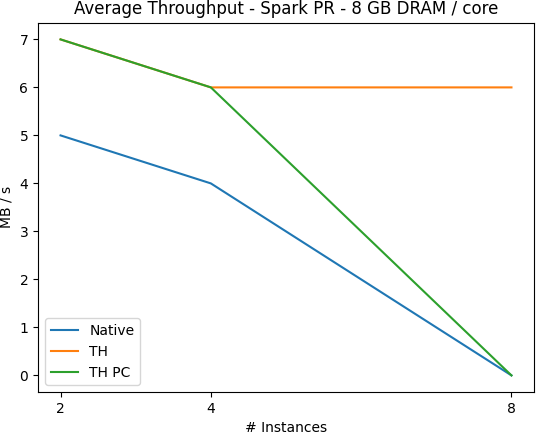
\includegraphics[width=\linewidth]{./fig/PR_64_THR.png}
    \caption{Native and TeraHeap Spark average throughput
	as the number of instances increases under 4 GB DRAM / core running Page Rank.}
\label{fig:pr_64_thr}
        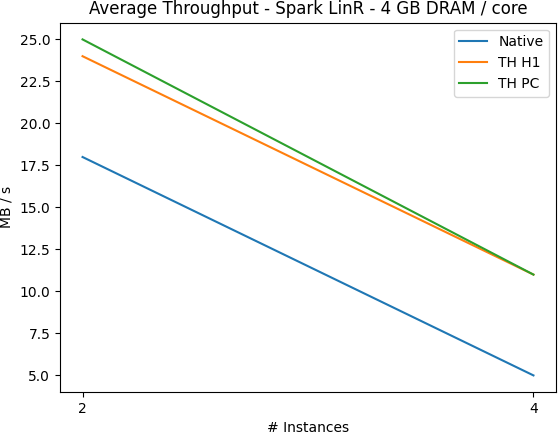
\includegraphics[width=\linewidth]{./fig/LINR_64_THR.png}
    \caption{Native and TeraHeap Spark average throughput
        as the number of instances increases under 4 GB DRAM / core running Linear Regression.}
                \label{fig:linr_64_thr}
\end{figure}

\begin{figure}[thbp]
	\centering
	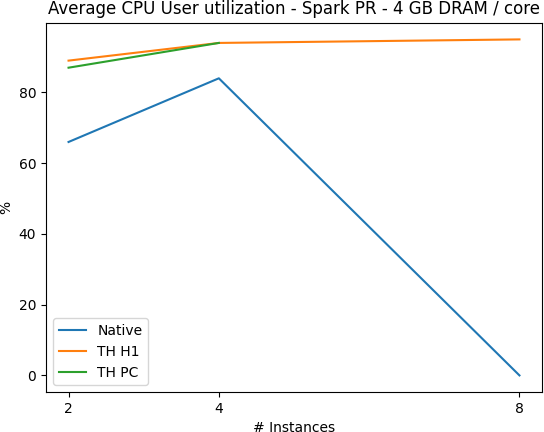
\includegraphics[width=\linewidth]{./fig/PR_64_USR.png}
    \caption{Native and TeraHeap Spark average user CPU utilization
        as the number of instances increases under 4 GB DRAM / core running Page Rank.}
		\label{fig:pr_64_usr}

	\centering
        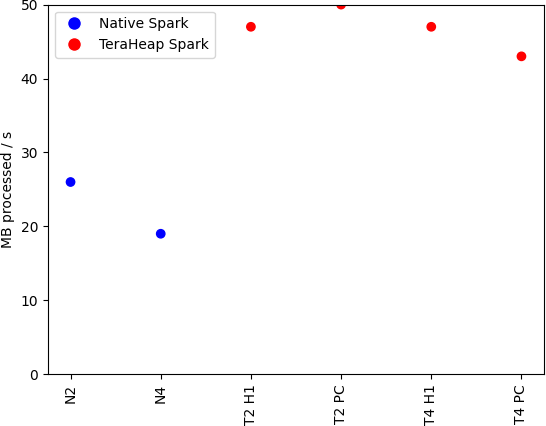
\includegraphics[width=\linewidth]{./fig/LOGR_64_THR.png}
    \caption{Native and TeraHeap Spark average throughput
        as the number of instances increases under 4 GB DRAM / core running Logistic Regression.}
		\label{fig:logr_64_thr}
\end{figure}

\begin{figure}[thbp]
	\centering
        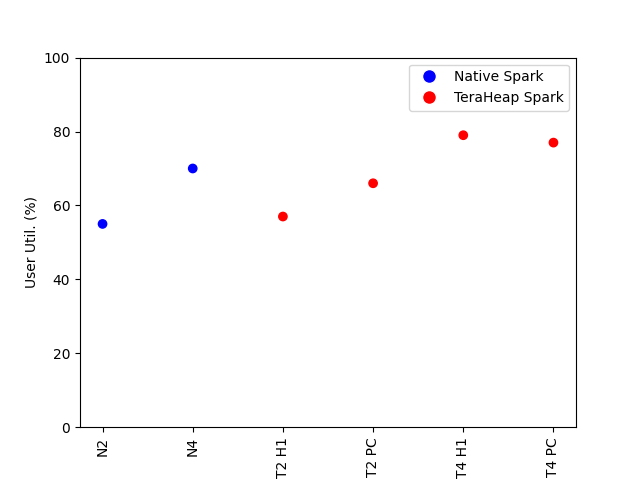
\includegraphics[width=\linewidth]{./fig/LINR_64_USR.png}
    \caption{Native and TeraHeap Spark average user CPU utilization
        as the number of instances increases under 4 GB DRAM / core running Linear Regression.}
		\label{fig:linr_64_usr}
    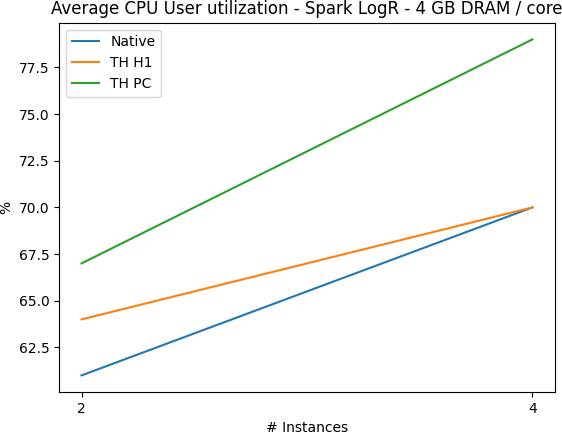
\includegraphics[width=\linewidth]{./fig/LOGR_64_USR.png}
    \caption{Native and TeraHeap Spark average user CPU utilization
        as the number of instances increases under 4 GB DRAM / core running Logistic Regression.}
	   \label{fig:logr_64_usr}
\end{figure}

\begin{figure}[thbp]
	\centering
        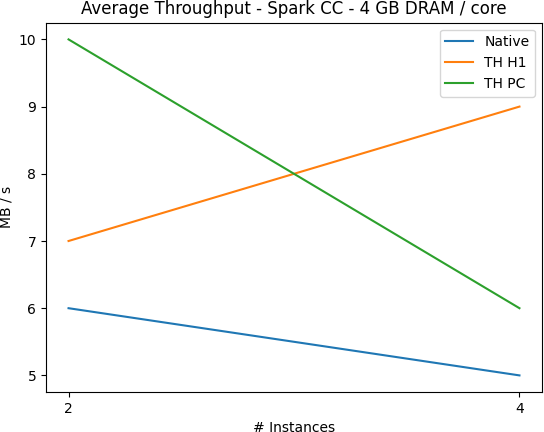
\includegraphics[width=\linewidth]{./fig/CC_64_THR.png}
    \caption{Native and TeraHeap Spark average throughput
        as the number of instances increases under 4 GB DRAM / core running Connected Component.}
		\label{fig:cc_64_thr}
        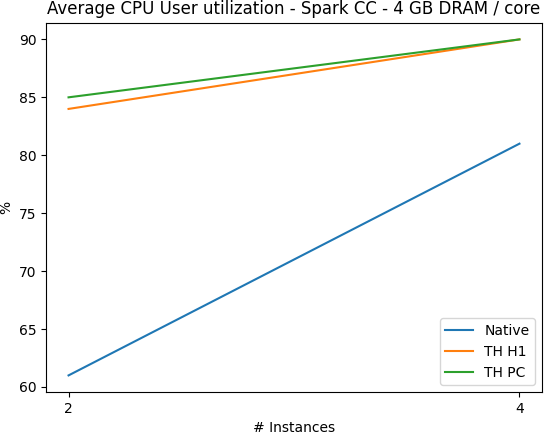
\includegraphics[width=\linewidth]{./fig/CC_64_USR.png}
    \caption{Native and TeraHeap Spark average user CPU utilization
        as the number of instances increases under 4 GB DRAM / core running Connected Component.}
	\label{fig:cc_64_usr}
\end{figure}

\begin{figure}[thbp]
	\centering
	\iffalse
        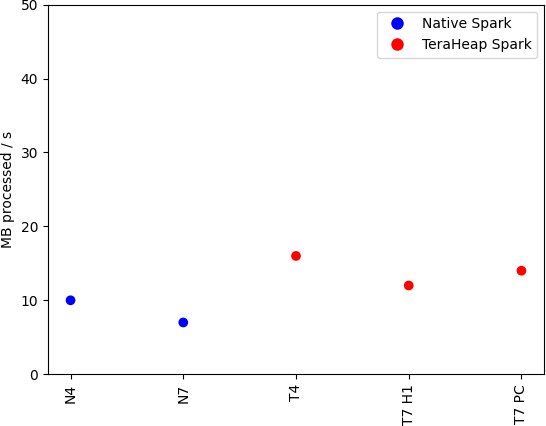
\includegraphics[width=\linewidth]{./fig/PR_256_THR.png}
    \caption{Page Rank 256 GB DRAM setup Native and TeraHeap
    throughput as the number of instances increases.Configurations
    starting with N denote a run with Native instances of Spark and
    with T with TeraHeap. H1 is a run with the memory budget
    configured to contain a bigger size for H1 than PageCache and PC
    the opposite. E.g. T2 PC is a run of 2 concurrent TeraHeap
    instances with exactly the same configuration. }
                \label{fig:pr_256_thr}
		\fi
        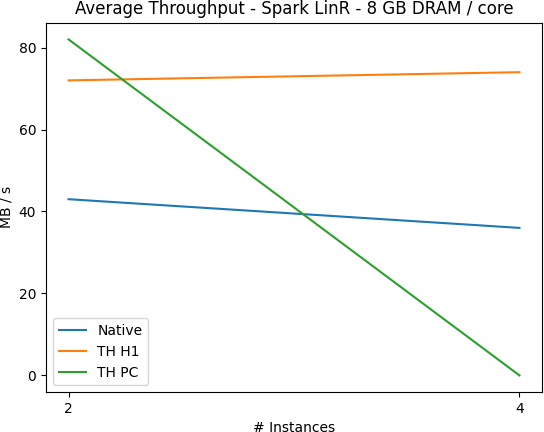
\includegraphics[width=\linewidth]{./fig/LINR_128_THR.png}
    \caption{Linear Regression 128 GB DRAM setup Native and TeraHeap
    throughput as the number of instances increases. Configurations
    starting with N denote a run with Native instances of Spark and
    with T with TeraHeap. H1 is a run with the memory budget
    configured to contain a bigger size for H1 than PageCache and PC
    the opposite. E.g. T2 PC is a run of 2 concurrent TeraHeap
    instances with exactly the same configuration.}
        \label{fig:linr_128_thr}
\end{figure}

\begin{figure}[thbp]
        \centering
	\iffalse
        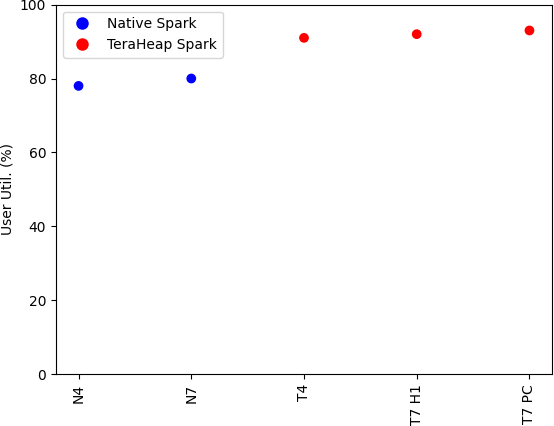
\includegraphics[width=\linewidth]{./fig/PR_256_USR.png}
    \caption{Page Rank 256 GB DRAM setup Native and TeraHeap
    User CPU utilization as the number of instances increases.Configurations
    starting with N denote a run with Native instances of Spark and
    with T with TeraHeap. H1 is a run with the memory budget
    configured to contain a bigger size for H1 than PageCache and PC
    the opposite. E.g. T2 PC is a run of 2 concurrent TeraHeap
    instances with exactly the same configuration. }
                \label{fig:pr_256_usr}
		\fi
        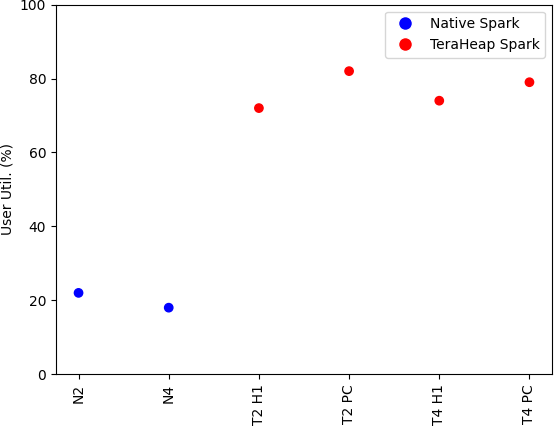
\includegraphics[width=\linewidth]{./fig/LINR_128_USR.png}
    \caption{Native and TeraHeap Spark average throughput
        as the number of instances increases under 8 GB DRAM / core running Linear Regression.}
        \label{fig:linr_128_usr}
\end{figure}


\begin{figure}[thbp]
        \centering
        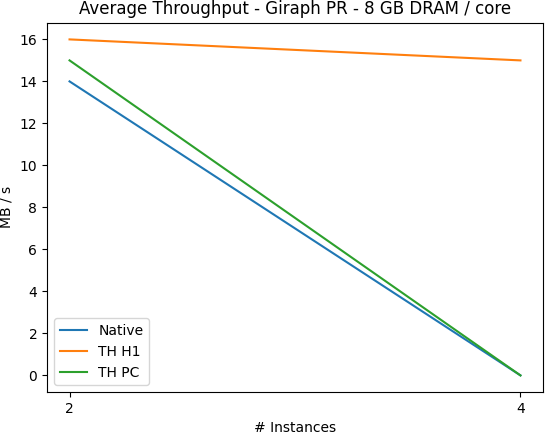
\includegraphics[width=\linewidth]{./fig/G_PR_128_THR.png}
    \caption{Native and TeraHeap Giraph average throughput
        as the number of instances increases under 8 GB DRAM / core running Page Rank.}
                \label{fig:g_pr_128_thr}
        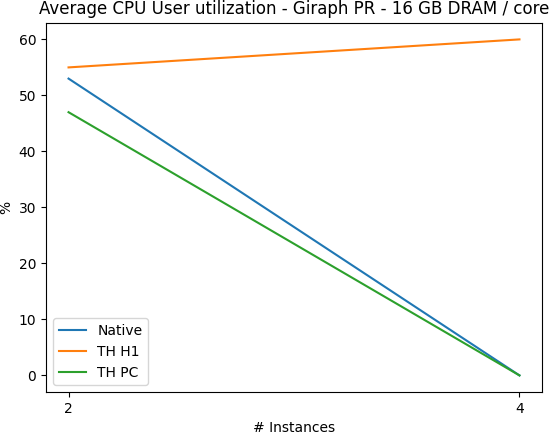
\includegraphics[width=\linewidth]{./fig/G_PR_128_USR.png}
    \caption{Native and TeraHeap Giraph average user CPU utilization
        as the number of instances increases under 8 GB DRAM / core running Page Rank.}
        \label{fig:g_pr_128_usr}
\end{figure}

\begin{figure}[thbp]
        \centering
        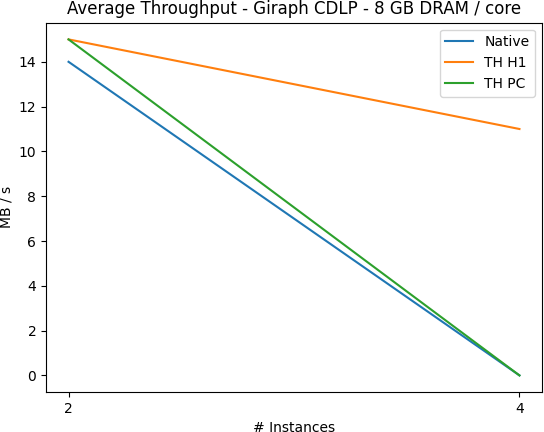
\includegraphics[width=\linewidth]{./fig/G_CDLP_128_THR.png}
    \caption{Native and TeraHeap Giraph average throughput
        as the number of instances increases under 8 GB DRAM / core running Page Rank.}
                \label{fig:g_cdlp_128_thr}
        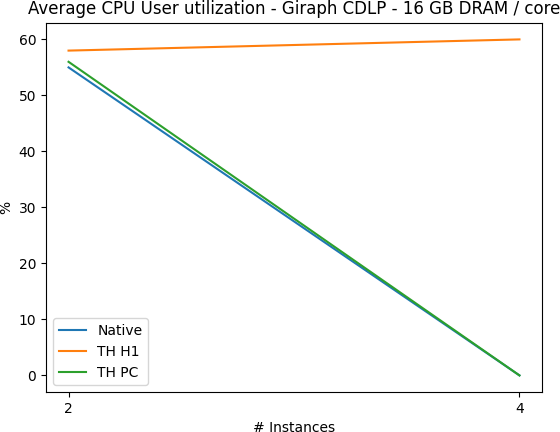
\includegraphics[width=\linewidth]{./fig/G_CDLP_128_USR.png}
    \caption{Native and TeraHeap Giraph average user CPU utilization
        as the number of instances increases under 8 GB DRAM / core running Page Rank.}
        \label{fig:g_cdlp_128_usr}
\end{figure}

\begin{table}[t!]
  \centering
  \caption{Range of increment between single and co-located \# of instances and corresponding range of increment factor of user CPU utilization}
  \label{tab:user_factors}
  \begin{tabular}{|c|c|}
    \hline
    \textbf{Incr. in # instances} & \textbf{Incr. Factor} \\
    \hline
    Native Spark 1 to 2  & 1.5x-2.5x \\
    Native Spark 1 to 4 & 2.5x \\
    TH Spark 1 to 2 & 2x-3x \\
    TH Spark 1 to 4 & 2x-3x \\
    Native Giraph 1 to 2 & 2x \\
    TH Giraph 1 to 2 & 2x-2.5x \\
    TH Giraph 1 to 4 & 2.5x-3x \\
    \hline
  \end{tabular}
\end{table}


The main goal for co-locating tasks is to increase the CPU utilization and achieve better
throughput. CPU utilization is split to 2 parts. 
User utilization includes all CPU cycles that were executed in user-space threads.
It includes GC cycles, S/D cycles and cycles for mutator tasks except I/O.
System utilization includes all CPU cycles that were executed in kernel-space threads.
This includes I/O carried out by GC (TeraHeap) and mutator I/O.
Therefore we have to focus to User utilization which includes the effective CPU cycles of the application.
By looking at figures \ref{fig:pr_64_usr}, \ref{fig:linr_64_usr},
\ref{fig:logr_64_usr}, \ref{fig:cc_64_usr} and \ref{fig:linr_128_usr} we see that Native and TeraHeap User CPU utiliztion
increases as the number of co-located instances of Spark increase in the server.
Table \ref{tab:user_factors} summarizes the increment of user CPU utilization for 1 to 2 and 1 to 4 instances for both offloading techniques.
The question that arises is if that User CPU utilization reflects the throughput in \ref{fig:pr_64_thr}, \ref{fig:linr_64_thr},
\ref{fig:logr_64_thr}, \ref{fig:cc_64_thr} and \ref{fig:linr_128_thr}. If comparing H1 and PC setups for TH we see that in Spark many times PC provides more average user CPU utlization. That is because GC increases and not because there is more work done by mutator threads. TH PC in \ref{fig:pr_64_thr} and \ref{fig:pr_64_usr} does not run OOM but there no more DRAM capacity in the machine to use a cgroup budget with more Page Cache size thus the line does not reach a final point. 0 MB / s throughput or 0\% user CPU utilization show that this experiment ran OOM.
From the figures of the previous section with the execution time breakdown and the User CPU Utilization of this section, we come to the conclusion that since TeraHeap has lower GC and S/D and higher CPU utilization the work by mutator threads for application tasks is higher.
For Native we see that the increment in CPU utilization is not useful work but more GC and S/D since the memory for each instance decreases as the number of co-located instances increase.

\subsection{What
happens with monetary cost across different cloud platforms?}

\iffalse
\begin{table}[htbp]
  \centering
	\begin{subtable}[b]{0.45\linewidth}
  \caption{Page Rank synopsis table. Configurations starting
    with N denote a run with Native instances of Spark and with T with
    TeraHeap. H1 is a run with the memory budget configured to contain
    a bigger size for H1 than PageCache and PC the opposite.}
  \label{tab:pr_table}
        %\resizebox{19cm}{!}{
        \begin{tabular}{|c|c|c|c|c|c|c|c|c|c|c|c|c|}
      \hline
\textbf{Conf.} & \textbf{H1 Size/I} & \textbf{Memory/I} & \textbf{Total Mem.} & \textbf{\#I} & \textbf{Exec. Time} & \textbf{CPU Idle} & \textbf{Total MB Proc.} & \textbf{MB/s} & \textbf{MB/s/I} & \textbf{Cost AWS \$} & \textbf{Cost GCP \$} & \textbf{Cost Azure \$} \\
        \hline
    N2 - small & 22 & 28 & 64 & 2 & 3563 & 29 & 16980 & 5 & 2 & 0.6 & 0.58 & 0.67 \\
    N4 - small & 11 & 14 & 64 & 4 & 8195 & 11 & 33960 & 4 & 1 & 1.8 & 1.74 & 2.01 \\
    T2 H1 – small & 22 & 28 & 64 & 2 & 2545 & 7 & 16980 & 7 & 3 & 0.6 & 0.58 & 0.67 \\
    T2 PC – small & 11 & 28 & 64 & 2 & 2385 & 9 & 16980 & 7 & 4 & 0.6 & 0.58 & 0.67 \\
    T4 H1 – small & 11 & 14 & 64 & 4 & 5554 & 1 & 33960 & 6 & 2 & 1.2 & 1.16 & 1.34 \\
    T4 PC – small & 6 & 14 & 64 & 4 & 5880 & 1 & 33960 & 6 & 2 & 1.2 & 1.16 & 1.34 \\
    N8 – small & 4 & 7 & 64 & 8 & OOM & ** & 0 & 0 & 0 & *** & *** & *** \\
    T8 – small & 4 & 7 & 64 & 8 & 12305 & 0 & 67920 & 6 & 1 & 2.4 & 2.32 & 2.68 \\
    N4 - big & 44 & 60 & 256 & 4 & 13542 & 15 & 135872 & 10 & 3 & 6.4 & *** & *** \\
    T4 – big & 48 & 60 & 256 & 4 & 9284 & 5 & 135782 & 16 & 4 \\      
	\hline
     \end{tabular}%
        %}
\end{subtable}

	\begin{subtable}[b]{0.45\linewidth}
  \caption{Linear Regression synopsis table. Configurations starting
    with N denote a run with Native instances of Spark and with T with
    TeraHeap. H1 is a run with the memory budget configured to contain
    a bigger size for H1 than PageCache and PC the opposite.}
  \label{tab:linr_table}
        %\resizebox{19cm}{!}{
        \begin{tabular}{|c|c|c|c|c|c|c|c|c|c|c|c|c|}
      \hline
\textbf{Conf.} & \textbf{H1 Size/I} & \textbf{Memory/I} & \textbf{Total Mem.} & \textbf{\#I} & \textbf{Exec. Time} & \textbf{CPU Idle} & \textbf{Total MB Proc.} & \textbf{MB/s} & \textbf{MB/s/I} & \textbf{Cost AWS \$} & \textbf{Cost GCP \$} & \textbf{Cost Azure \$} \\
	\hline 
      N2 & 22 & 28 & 64 & 2 & 3745 & 20 & 134896 & 37 & 18 & 0.6 & 0.58 & 0.67 \\ 
      N4 & 11 & 14 & 64 & 4 & 13874 & 7 & 269792 & 20 & 5 & 2.4 & 2.32 & 2.01 \\
      T2 H1 & 22 & 28 & 64 & 2 & 2891 & 19 & 134896 & 48 & 24 & 0.6 & 0.58 & 0.67 \\
      T2 PC & 11 & 28 & 64 & 2 & 2747 & 18 & 134896 & 49 & 25 & 0.6 & 0.58 & 0.67 \\
      T4 H1 & 11 & 14 & 64 & 4 & 6075 & 2 & 269792 & 44 & 11 & 1.2 & 1.16 & 1.34 \\
      T4 PC & 6 & 14 & 64 & 4 & 6176 & 3 & 269792 & 44 & 11 & 1.2 & 1.16 & 1.34 \\ 
      \hline
     \end{tabular}%
	%}
\end{subtable}
	\vspace{1em}
\end{table}
\fi
\iffalse
%\begin{center}%[htbp]
 %   \centering
  %  \caption{Page Rank synopsis table}
\begin{table*}
\resizebox{\textwidth}{!}{
\begin{tabular}{|c|c|c|c|c|c|c|c|c|c|c|c|c|c|c|c|c|}
		%\begin{tabularx}{\linewidth}{*{17}{X}}
	    \hline
        \multirow{2}{*}{Configuration} & H1       & \multirow{2}{*}{Mem / I} & Total & \multirow{2}{*}{\#I} & Exec. & User  & System & I/O  & CPU  & Total MB  & \multirow{2}{*}{MB/s} & \multirow{2}{*}{MB/s/I} & Cost   & Cost   & Cost \\
                                       & Size / I &                          & memory &                     & Time  & util. & util.  & Wait & Idle & Processed &                       &                         & AWS \$ & GCP \$ & Azure \$ \\
        \hline
        \hline
        N2-small – single & 22 & 28 & 64 & 1 & 1762 & 32 & 2 & 1 & 65 & 8490 & 5 & 5 & 0.6 & 0.58 & 0.67 \\
        N2 - small & 22 & 28 & 64 & 2 & 3563 & 66 & 5 & 2 & 27 & 16980 & 5 & 2 & 0.6 & 0.58 & 0.67 \\
        N4 – small – single & 11 & 14 & 64 & 1 & 1783 & 29 & 2 & 1 & 68 & 8490 & 5 & 5 & 0.6 & 0.58 & 0.67 \\
        N4 - small & 11 & 14 & 64 & 4 & 8195 & 84 & 6 & 2 & 8 & 33960 & 4 & 1 & 1.8 & 1.74 & 2.01 \\
        N8 – small & 4 & 7 & 64 & 8 & OOM & 0 & 0 & 0 & ** & 0 & 0 & 0 & *** & *** & *** \\
        T2 H1- small – single & 22 & 28 & 64 & 1 & 1146 & 46 & 2 & 1 & 51 & 8490 & 7 & 7 & 0.6 & 0.58 & 0.67 \\
        T2 H1 – small & 22 & 28 & 64 & 2 & 2545 & 89 & 4 & 1 & 6 & 16980 & 7 & 3 & 0.6 & 0.58 & 0.67 \\
        T2 PC- small – single & 11 & 28 & 64 & 1 & 966 & 45 & 2 & 1 & 52 & 8490 & 9 & 9 & 0.6 & 0.58 & 0.67 \\
        T2 PC – small & 11 & 28 & 64 & 2 & 2385 & 87 & 4 & 0 & 9 & 16980 & 7 & 4 & 0.6 & 0.58 & 0.67 \\
        T4 H1 – small – single & 11 & 14 & 64 & 1 & 984 & 43 & 3 & 1 & 53 & 8490 & 9 & 9 & 0.6 & 0.58 & 0.67 \\
        T4 H1 – small & 11 & 14 & 64 & 4 & 5554 & 94 & 5 & 0 & 1 & 33960 & 6 & 2 & 1.2 & 1.16 & 1.34 \\
        T4 PC – small – single & 6 & 14 & 64 & 1 & 922 & 42 & 2 & 2 & 54 & 8490 & 9 & 9 & 0.6 & 0.58 & 0.67 \\
        T4 PC – small & 6 & 14 & 64 & 4 & 5880 & 94 & 5 & 0 & 1 & 33960 & 6 & 2 & 1.2 & 1.16 & 1.34 \\
        T8 – small – single & 4 & 7 & 64 & 1 & 1037 & 39 & 2 & 1 & 58 & 8490 & 8 & 8 & 0.6 & 0.58 & 0.67 \\
        T8 – small & 4 & 7 & 64 & 8 & 12305 & 95 & 5 & 0 & 0 & 67920 & 6 & 1 & 2.4 & 2.32 & 2.68 \\
        N4 - big & 48 & 60 & 256 & 4 & 13542 & 78 & 7 & 7 & 8 & 135872 & 10 & 3 & 6.4 & *** & *** \\
        T4 – big & 48 & 60 & 256 & 4 & 9284 & 91 & 8 & 1 & 1 & 135782 & 16 & 4 & 1.8 & *** & *** \\
        \hline
	\bottomrule
\end{tabular}
}
\end{table*}
%	\label{tab:pr_table}
%\end{center}
\fi
\iffalse
\begin{table}[t!]
  \centering
  \caption{Logistic Regression synopsis table. Configurations starting
    with N denote a run with Native instances of Spark and with T with
    TeraHeap. H1 is a run with the memory budget configured to contain
    a bigger size for H1 than PageCache and PC the opposite.}
  \label{tab:logr_table}
	\resizebox{19cm}{!}{
	\begin{tabular}{|c|c|c|c|c|c|c|c|c|c|c|c|c|}
      \hline
\textbf{Conf.} & \textbf{H1 Size/I} & \textbf{Memory/I} & \textbf{Total Mem.} & \textbf{\#I} & \textbf{Exec. Time} & \textbf{CPU Idle} & \textbf{Total MB Proc.} & \textbf{MB/s} & \textbf{MB/s/I} & \textbf{Cost AWS \$} & \textbf{Cost GCP \$} & \textbf{Cost Azure \$} \\
      \hline
      N2 & 22 & 28 & 64 & 2 & 5127 & 18 & 133348 & 26 & 13 & 1.2 & 1.16 & 0.67 \\
      N4 & 11 & 14 & 64 & 4 & 13730 & 7 & 266696 & 19 & 5 & 2.4 & 2.32 & 2.68 \\
      T2 H1 & 22 & 28 & 64 & 2 & 2861 & 18 & 133348 & 47 & 24 & 0.6 & 0.58 & 0.67 \\
      T2 PC & 11 & 28 & 64 & 2 & 2683 & 18 & 133348 & 50 & 25 & 0.6 & 0.58 & 0.67 \\
      T4 H1 & 10 & 14 & 64 & 4 & 5712 & 2 & 266696 & 47 & 12 & 1.2 & 1.16 & 1.34 \\
      T4 PC & 6 & 14 & 64 & 4 & 6138 & 2 & 266696 & 43 & 10 & 1.2 & 1.16 & 1.34 \\
      \hline
     \end{tabular}%
	}
\end{table}

\begin{table}[t!]
  \centering
  \caption{Connected Component synopsis table. Configurations starting
    with N denote a run with Native instances of Spark and with T with
    TeraHeap. H1 is a run with the memory budget configured to contain
    a bigger size for H1 than PageCache and PC the opposite.}
  \label{tab:cc_table}
        \resizebox{19cm}{!}{
        \begin{tabular}{|c|c|c|c|c|c|c|c|c|c|c|c|c|}
      \hline
\textbf{Conf.} & \textbf{H1 Size/I} & \textbf{Memory/I} & \textbf{Total Mem.} & \textbf{\#I} & \textbf{Exec. Time} & \textbf{CPU Idle} & \textbf{Total MB Proc.} & \textbf{MB/s} & \textbf{MB/s/I} & \textbf{Cost AWS \$} & \textbf{Cost GCP \$} & \textbf{Cost Azure \$} \\
	\hline
      N2 & 22 & 28 & 64 & 2 & 2958 & 26 & 16980 & 6 & 3 & 0.6 & 0.58 & 0.67 \\
      N4 & 11 & 14 & 64 & 4 & 7231 & 7 & 33960 & 5 & 3 & 1.8 & 1.74 & 2.01 \\
      T2 H1 & 22 & 28 & 64 & 2 & 2526 & 5 & 16980 & 7 & 4 & 0.6 & 0.58 & 0.67 \\
      T2 PC & 11 & 28 & 64 & 2 & 2519 & 7 & 16980 & 7 & 4 & 0.6 & 0.58 & 0.67 \\
      T4 H1 & 11 & 14 & 64 & 4 & 5439 & 3 & 33960 & 6 & 3 & 1.2 & 0.58 & 0.67 \\
      T4 PC & 6 & 14 & 64 & 4 & 5487 & 2 & 33960 & 6 & 3 & 1.2 & 1.16 & 1.34 \\
      \hline
     \end{tabular}%
	}
\end{table}
\fi


\begin{table}[t!]
  \centering
  \caption{Hourly costs for EC2, GCP and Azure Cloud}
  \label{tab:cost_table}
  \begin{tabular}{|c|c|c|c|}
    \hline
	  \textbf{Provider} & \textbf{DRAM (GB)} & \textbf{Cores #} & \textbf{Hourly cost (\$)} \\
    \hline
	  EC2 & 128 & 16 & 0.72  \\
	  EC2 & 64 & 16 & 0.6 \\
	  GCP & 128 & 16 & 0.8  \\
	  GCP & 64 & 16 & 0.58 \\
	  AZ & 128 & 16 & 0.99 \\
	  AZ & 64 & 16 & 0.67 \\
    \hline
  \end{tabular}
\end{table}


Tables \ref{tab:cost_table} shows hourly cost for each machine configuration in 
Amazon Web Services Cloud (EC2), GCP (Google Cloud Platform) and Microsoft Azure costs. 
We witness that Amazon and Google providers offer a similar cost for identical machines to our server.
Azure is more expensive especially for the 8 GB memory / core machine where it is 20\% more expensive than GCP.
Taking into account that we have an hourly cost,
TeraHeap could be used for running colocated Spark and Giraph workloads
and achieve benefits of up to 50\%. The calculations are very simple so we skip them. We multiple hourly cost
by number of hours needed to execute each experiment until all instances finish execution. The conclusion is that reducing GC and S/D makes a huge difference in the execution time and therefore running with TeraHeap decreases the hours needed to rent the machines.

